\input{../../Plantillas-Fomato/Tareas/tarea.tex}
\cabe{Geometría 3: Tarea 3}{Jhonny Lanzuisi, 1510759}

\begin{document}
		\thispagestyle{plain}
		\tituloD{Geometría 3}{Tercera Tarea}
		\subsection*{Ejercicio 1}
		Sea $\bigtriangleup ABC$ un triángulo y sean $A\prime, B'$ y $C'$ sobre los lados $a$, $b$ y
		$c$, respectivamente. Mostrar que las circunferencias que pasan por los
		puntos $AC'B'$ , $A'BC'$ y $A'B'C$ concurren en un mismo punto $P$.
		
		\begin{sol}
		Supongamos que las circunferencias $AC'B'$ y $A'BC'$ se cortan en un punto $P$ distinto de $A$. Entonces los cuadriláteros $AB'PC'$ y $BA'PC'$ estan inscritos en las circunferencias $AC'B'$ y $A'BC'$ respectivamente, por lo que los ángulos opuestos de estos dos cuadriláteros son suplementarios. Se tiene entonces que
		\begin{align*}
			\angle A'PB' &= 2\pi-\angle C'PA'-\angle C'PB' \\
						 &= 2\pi - (\pi-\angle C'BA') - (\pi-\angle C'AB') \\
						 &= \angle C'BA' + \angle C'AB' \\
						 &= \pi-\angle A'CB'.
		\end{align*}
		
		Por el razonamiento anterior el ángulo $\angle A'PB'$ es el suplementario del ángulo $\angle A'CB'$. Como estos ángulos son suplementarios el cuadrilátero \linebreak$A'CB'P$ esta inscrito en la circunferencia $A'CB'$ y corta con las otras dos en $P$, como se buscaba.
		\begin{figure}[H]\centering
			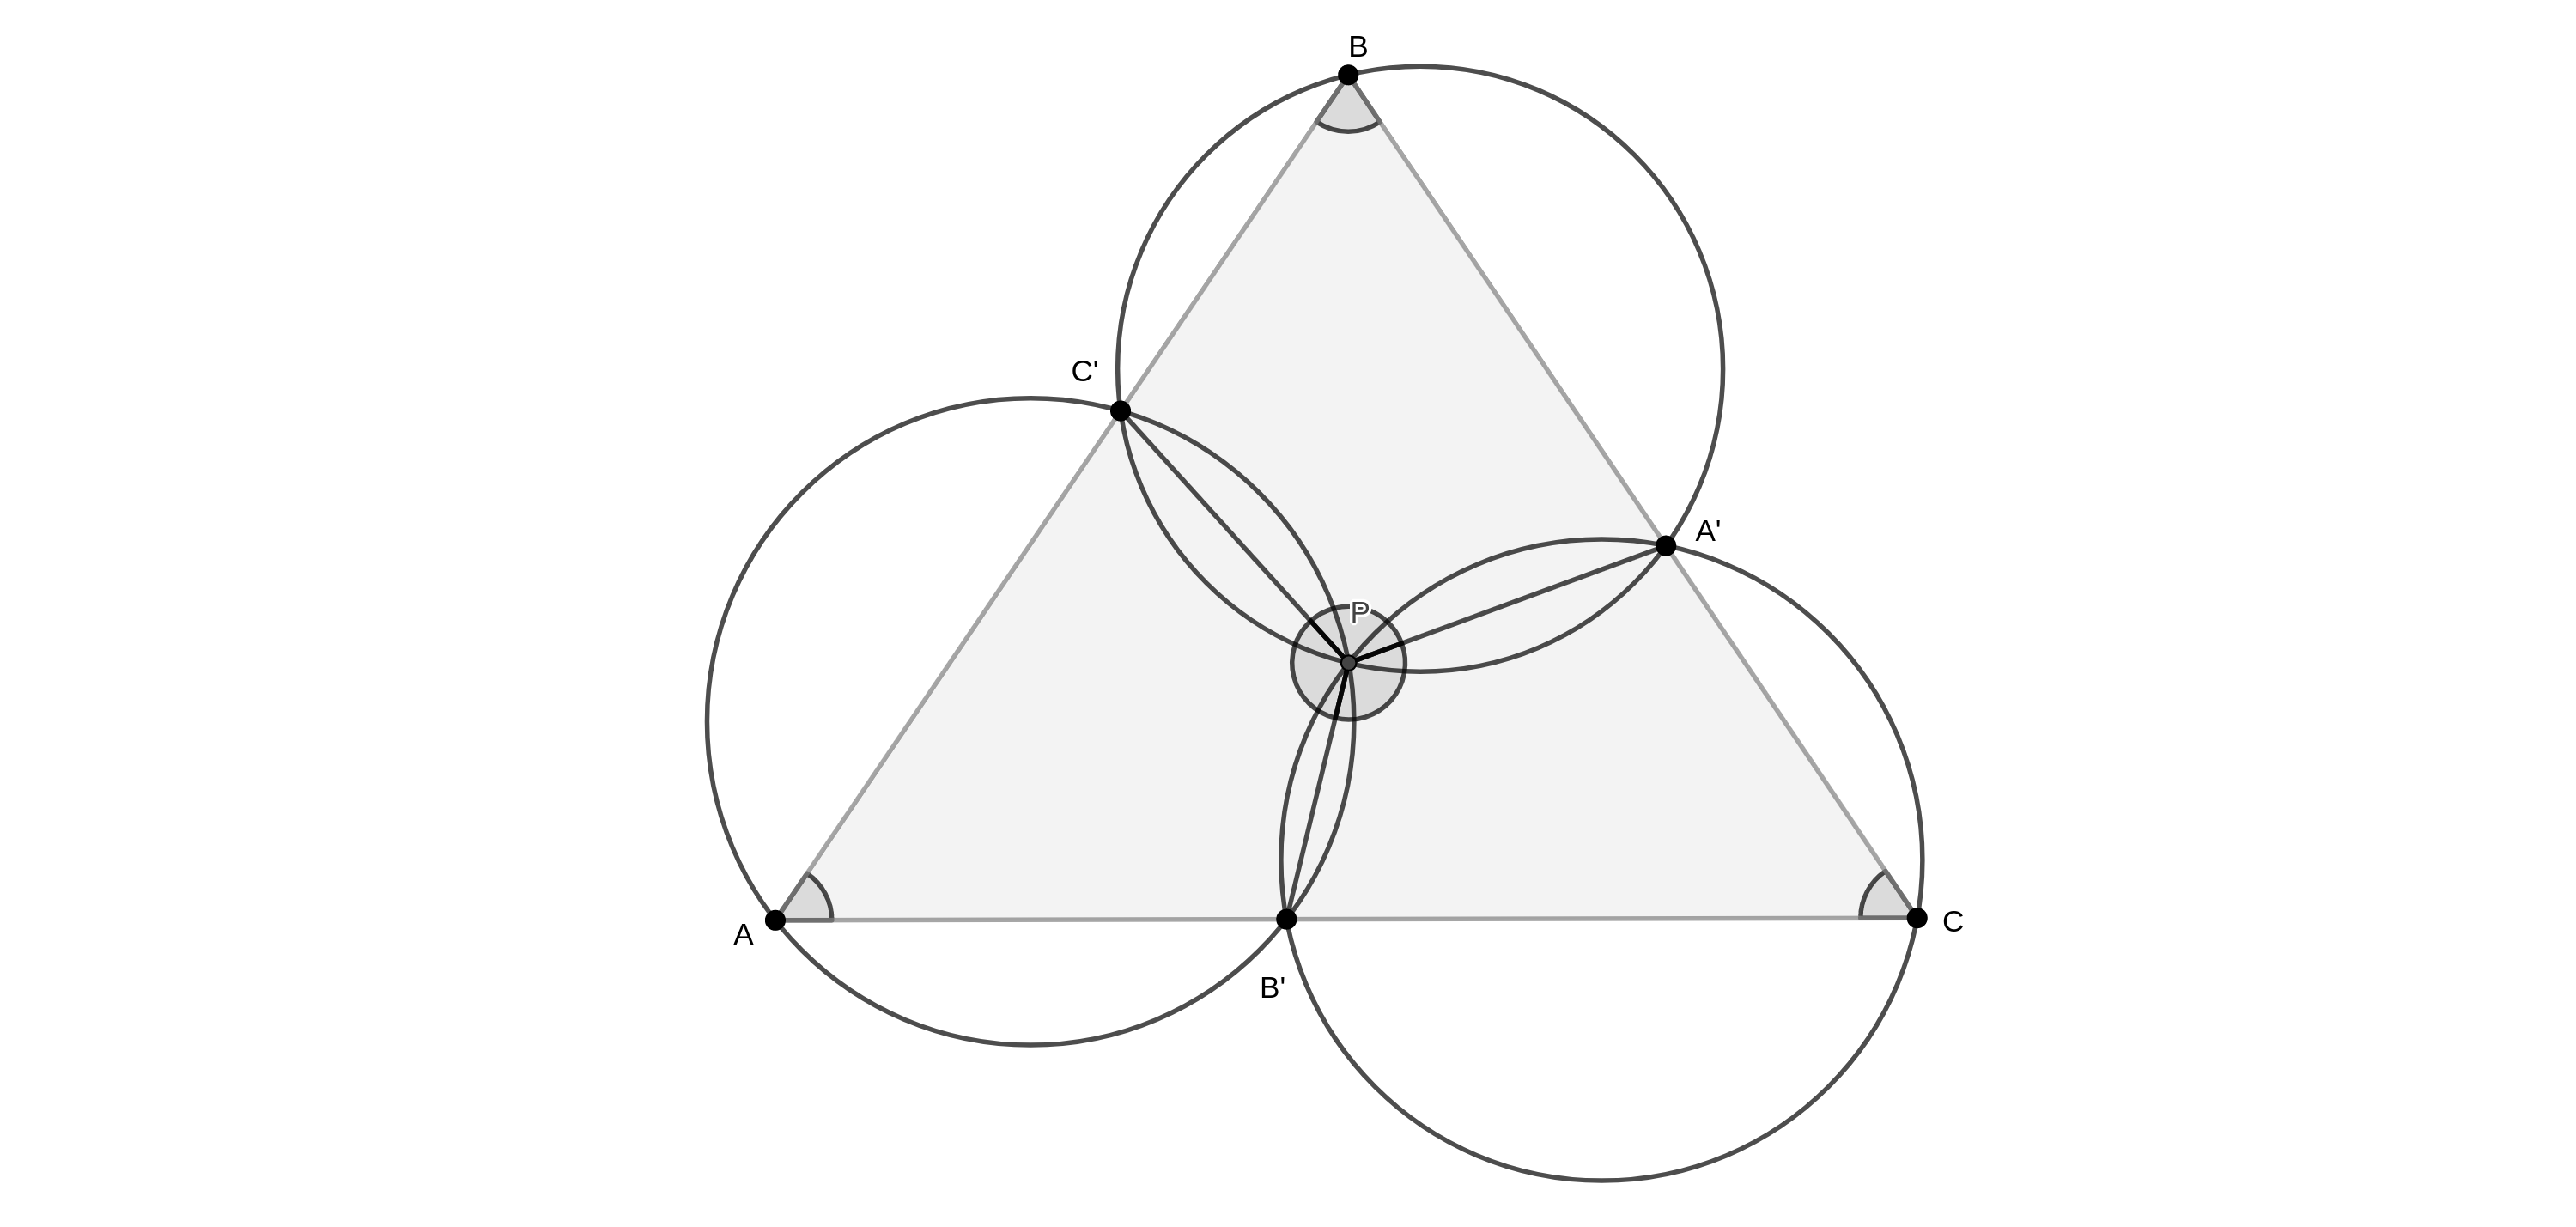
\includegraphics[width=1\linewidth]{pics/g4}
		\end{figure}
		\end{sol}
%	\subsection{Ejercicio 2}
%	Dados cuatro puntos en el plano y un ángulo, hallar un rombo que
%	pase por dichos puntos y tal que el ángulo formado por dos de sus lados
%	coincida con el ángulo dado.
%	\begin{sol}
%	Sean $A,B,C$ y $D$ dado así como el ángulo $\alpha$ . Coloquemos el ángulo $\alpha$ en el punto $A$, los vertices del rombo se encuentran en el arco capaz de segmento $PS$ y ángulo
%	$\alpha$ . Por otra parte podemos considerar la diagonal AT como lado del ángulo inscrito
%	]PAT en dicho arco capaz y valor α 2 . Hallando el ángulo central correspondiente,
%	su intersección con la circunferencia que contiene al arco capaz nos proporciona
%	el punto T de dicha diagonal. Procediendo análogamente con los otros tres arcos
%	capaces y hallando las diagonales, sus intersecciones con los arcos capaces nos dan
%	los vértices del rombo
%	\end{sol}
%\usetikzlibrary{arrows}
%\definecolor{uuuuuu}{rgb}{0.26666666666666666,0.26666666666666666,0.26666666666666666}
%\definecolor{qqwuqq}{rgb}{0,0.39215686274509803,0}
%\definecolor{ududff}{rgb}{0.30196078431372547,0.30196078431372547,1}
%\begin{tikzpicture}[line cap=round,line join=round,>=triangle 45,x=1cm,y=1cm]
%\clip(-10.846511712155884,-2.837516177094496) rectangle (6.402591952275694,5.382957091972081);
%\draw [shift={(-7.36,-1.11)},line width=2pt,color=qqwuqq,fill=qqwuqq,fill opacity=0.10000000149011612] (0,0) -- (-3.4556937180918377:0.3788236529523773) arc (-3.4556937180918377:45:0.3788236529523773) -- cycle;
%\draw [line width=2pt,domain=-10.846511712155884:6.402591952275694] plot(\x,{(--14.375--2.3*\x)/2.3});
%\draw [line width=2pt,domain=-10.846511712155884:6.402591952275694] plot(\x,{(-12.8708-0.5*\x)/8.28});
%\draw [line width=2pt,domain=-10.846511712155884:6.402591952275694] plot(\x,{(--20.4326--8.28*\x)/0.5});
%\draw [line width=2pt,domain=-10.846511712155884:6.402591952275694] plot(\x,{(--3.749--2.3*\x)/-2.3});
%\draw [line width=2pt] (-2.2246272493573263,4.025372750642672)-- (-0.08041131105398538,-1.549588688946015);
%\draw (-3.9645486835210306,-1.4990059366627646) node[anchor=north west] {\textit{b}};
%\draw (-5.000000001590862,1.7336225685308508) node[anchor=north west] {\textit{c}};
%\draw (-0.795057453819474,1.1906419992991106) node[anchor=north west] {$a$};
%\begin{scriptsize}
%\draw [fill=ududff] (-7.36,-1.11) circle (2.5pt);
%\draw[color=ududff] (-7.260314464206712,-0.8360645439961053) node {$A$};
%\draw [fill=ududff] (-2.42,0.79) circle (2.5pt);
%\draw[color=ududff] (-2.3229795207273956,1.0580537207657787) node {$H$};
%\draw [fill=uuuuuu] (-2.2246272493573263,4.025372750642672) circle (2pt);
%\draw[color=uuuuuu] (-2.4492540717115214,4.240172405565744) node {$B$};
%\draw [fill=uuuuuu] (-0.08041131105398538,-1.549588688946015) circle (2pt);
%\draw[color=uuuuuu] (0.02572712757734343,-1.3032803826373702) node {$C$};
%\end{scriptsize}
%\end{tikzpicture}
\end{document}